\documentclass[12pt]{article}
\usepackage{amsmath}
\usepackage{amssymb}
\usepackage{geometry}
\usepackage{enumerate}
\usepackage{natbib}
\usepackage{float}%稳定图片位置
\usepackage{graphicx}%画图
\usepackage[english]{babel}
\usepackage{a4wide}
\usepackage{indentfirst}%缩进
\usepackage{enumerate}%加序号
\usepackage{multirow}%合并行


\begin{document}
\newpage
\section{Answers for Pre Lab Questions}
\subsection{Question 1}
\begin{figure}[H]
\centering
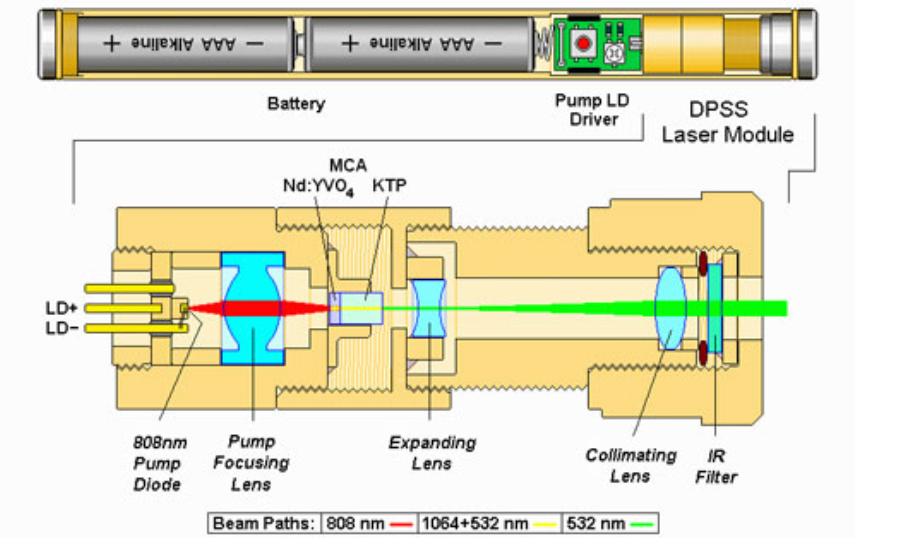
\includegraphics[scale=0.5]{P1.png}
\end{figure}
This is a schematic diagram of a green laser pointer. The two AAA Alkaline batteries can provide voltage for the pump LD driver which can drive the pump diode to produce red laser with wavelength at 808nm. Then the pump focusing lens can focus the red laser to the $YVO_s$ to produce red laser with wavelength at 1064nm. After going through the expanding lends, the laser's wavelength will be half of its origin value through second harmonic generation, which is 532nm so it's green laser. Then the collimating lens can make the light horizontal and the IR filter can prevent long wavelength laser from shooting to make the pointer harmless.
\subsection{Question 2}
When the phase is matched, the difference of wavelength of two light is zero, $\Delta k=k_2-2k_1=0$, where $2k_1=\frac{2\omega n_1}{c}$, $k_2=\frac{2\omega n_2}{c}$. So the refractive index of two medium should be same. When the medium is aniaxial negative crystal, $n_o^\omega\leq n_e^{2\omega}$, when it's uni-axial crystal, $n_e^{\omega}\leq n_o^{2\omega}$
\par Assume $\theta_m$ is the matching angle, when it's type-I matching, for niaxial negative crystal, $n_o^{\omega}=n_e^{2\omega}(\theta_m)$. For uni-axial crystal, $n_o^{2\omega}=n_e^{\omega}(\theta_m)$. When it's type-II matching, for niaxial negative crystal, $2n_e^{2\omega}(\theta_m)=n_e^{\omega}(\theta_m)+n_o^{\omega}$. For uni-axial crystal, $2n_o^{2\omega}=n_e^{\omega}(\theta_m)+n_o^{\omega}$.
\end{document}